%\documentclass[a4paper]{article}
\documentclass[10pt,journal,letterpaper,twocolumn]{IEEEtran}

\usepackage[english]{babel}
\usepackage[utf8]{inputenc}
\usepackage{amsmath}
\usepackage{graphicx}
\usepackage{array}
\usepackage[table]{xcolor}
\usepackage{float}
\usepackage[colorinlistoftodos]{todonotes}
\usepackage{cite}

\floatstyle{plaintop}
\restylefloat{table}

\setlength{\arrayrulewidth}{1mm}
\setlength{\tabcolsep}{6pt}
\renewcommand{\arraystretch}{2}

\title{Making a Smarter Microwave}

\author{Stuart Johnsen, Darin Stoker, James Watts\\University of Utah\\ Department of Electrical and Computer Engineering}

\date{\today}

\begin{document}

\maketitle

\begin{abstract}
The planning and implementation of a smart microwave is discussed. The main components of the project are dissected, including the microwave modifications, the hardware bridge construction, the Android application code, and the Arduino sketch code.  Challenges in completing the project are discussed, as are potential future improvements.
\end{abstract}

\section{Introduction}
As  electronic technology is increasingly incorporated into aspects of daily life, one of the last remaining product families that has been nearly untouched by the technology's advance has been in the kitchen.  Particularly,  advances in microwave oven technology has stagnated, even as other fields of technology have advanced ease and life comfort.   Some of this is due simply to the the simplicity of microwaves; they are not particularly complex devices.  The overall circuitry for controlling a microwave is virtually identical to its first inceptions, and this reliability and simplicity has made it easy for microwave manufacturers to pump them out at low cost, with little incentive to make them "smarter" or user friendly.  Simple microcontrollers have been added over the years, and basic improvements to user interfaces have been made, but in relation to the improvements being made in user interfaces, databases, and other technologies have not translated to direct use in the kitchen.

\subsection{Motivation}
In researching the background and history of microwave ovens, we found that the aesthetic and user-friendly qualities of microwaves have only been lightly improved upon since they became household items.  While digital interfaces became common for readouts and button presses, the overall way that people interact with microwaves has not changed in many years.  And even though microwaves are pretty ubiquitous items, we found that even we as engineers did not understand how they worked or why the seemingly un-resolvable problems with microwaves have lingered on.

In our research, we found that microwaves were not incredibly complex devices, nor were those "un-resolvable" problems all that difficult to solve.  Even with our student engineer credentials, we found that we ourselves could take a stab at making the microwave more user friendly.  Using a combination of hardware engineering and computer science, we decided to make a "smarter" microwave.

\subsection{Proposal}
We propose a solution to upgrade the currently outdated technology found in microwave, specifically in relation to the user interface and ease of use.  Using a combination of software application development and embedded systems engineering, we have developed a prototype system to increase the capabilities of the household microwave, including the following upgrades:

\begin{enumerate}
\item An update-able database of entries containing information on food items and encoded instructions for cooking them.
\item An Android application to control the microwave, comprising of:
\begin{enumerate}
	\item A connection to the food information database.
    \item Multiple modes for cooking food based based on user input or on database instructions.
    \item A method for manually searching the database for the desired entry.
    \item A method to search the database by scanning a UPC bar code.
    \item A set of software timer synced with the microwave timer.
    \item An Android application GUI based on states and activities.
    \item Software to send information to the hardware via USB.
\end{enumerate}
\item An Arduino embedded system to control the hardware system, comprising of:
\begin{enumerate}
	\item An embedded interrupt system to recognize received data from the serial connection.
    \item Instructions to decode the instruction strings coming from the Android application \cite{raspberryPicrowaveRepo}.
    \item A method of re-connecting to the tablet if connection is lost.
    \item Methods to control the external hardware and the microwave itself.
\end{enumerate}
\item A hardware system to control the microwave's functionality via replicating user button presses.  Our system replicates button presses via a set of hardware relays.
\item Hardware to control the plate spinning within the microwave.
\item Hardware to control airflow within the microwave and prevent condensation.
\item A thermal camera to view the heating process within the microwave.
\end{enumerate}

\begin{figure*}[ht]
\centering
\includegraphics[width=\textwidth]{HardwareSoftware.png}
\caption{\label{fig:hardwaresoftware}Figure displaying the software/hardware communication.}
\end{figure*}

\subsection{General Project Overview}
This multi-approach system helps bring the microwave into the modern day.  At its heart is the Android application, which acts as the main user interface and is the centerpiece of the implementation.  Its primary behind-the-scenes function is that it connects the microwave to a database containing information about microwavable foods, making cooking foods more predictable and reliable.  Table~\ref{tab:database} in the appendix shows the structure of the database that we built.
From the database, the Android application separates out the necessary information that needs to be displayed to the user and what needs to be sent to the microwave.  Via either of the "search by name" or "search by UPC" activities shown in Figure \ref{fig:activitymap}, the user can select the food to be cooked, see a picture of it and the necessary cooking steps, and program the microwave.  From there, the application takes over, sending instructions to the hardware to begin cooking, and it starts a timer to keep track of the food's cooking time in sync with the microwave.  Finally, once the food is cooked, the user can reset the application by traversing back through the activities, and can enjoy their food.  More on this will be explained in further sections.

Our original aim for the project was to also include image processing based on input from the thermal camera.  Unfortunately, the company with whom we were working was unable to provide us with the necessary software development kit on time, so we were unable to include the image processing capabilities we originally planned for.  As such, we had to modify our original aims of the project and omit the image processing.  We will explain more of this idea in the further implementation section.

Once the information is parsed from the database, hardware translates the information coming from the Android into replicated button presses on the microwave.  We did not modify the existing microwave hardware controls in order to preserve safety features, such as over-current protections, already built into the microwave.  The Arduino is connected to the android application via a serial communication link over USB.  The instructions sent from the Android application are then decoded by the Arduino as shown in Figure \ref{fig:decodinginstructions}, coded into button presses and sent to the relay board \cite{raspberryPicrowaveRepo}.  By leveraging the flexible nature of the relay board, we also implemented methods to control the microwave's plate spinning, and added an external fan for ventilation.  The full map of how the software and hardware systems interact is shown in Figure \ref{fig:hardwaresoftware}.

\section{Hardware}
With the overview of the project given, the following sections will go over the steps that we took in creating our prototype smart microwave, starting with understanding the microwave itself.

\subsection*{Microwave Components}
The first step in starting to understand where to start building our solution was to first understand how the microwave worked in order to design a hardware harness to control the microwave.  As our prototype base, we bought a popular, cheap, low end WestBend branded microwave.  The basic components of the microwave are shown in Figure \ref{fig:innards}, and include all the basic active parts of a microwave:

\begin{itemize}
    \item The magnetron - the component of the microwave that converts an electrical source into the microwaves that heat food.
    \item A transformer - There is a large transformer for the magnetron alone that steps up the voltage massively in order to convert project electrons into the microwave enclosure.  As the magnetron requires a DC power supply, the transformer works in conjunction with a very large capacitor (also shown) in order to maintain a steady DC source.  There is also a smaller transformer in the back of the microwave which does a AC-DC conversion for the controller board.
    \item The controller board and button panel- Located behind the button panel of the microwave sits the microwave's controller board and supporting componentry.  The buttons on the microwave front panel link directly to this board, which does all the necessary work.
    \item Plate motor - Underneath the main enclosure is a mounted motor that comes up through the bottom of the main enclosure box and spins the interior food plate.  In testing it, we found the motor to be extremely well self-contained, with the necessary support circuitry to handle start-up current and torque.
    \item Fan - At the rear of the microwave component area is a fan that helps to keep the power components from overheating.
\end{itemize}

All the included active componentry was grounded to the shell of the microwave, which in turn is grounded to the input ground line.

\begin{figure}[ht]
\centering
\includegraphics[width=0.4\textwidth]{Microwave_Innards.jpeg}
\caption{\label{fig:innards}Picture showing the basic components of a microwave.}
\end{figure}

\subsection*{Microcontroller and Button Decoding}

The next task was to remove the protective components of the microwave like the outer casing and the securing components in order to access the microwave microcontroller and button panel.  Figure \ref{fig:innards} above shows the interior componentry area after we removed the outer casing.  From there, we were able to remove the microwave controller board from the front button panel and identify the type of microcontroller being used, a Sino Wealth SH69P26.  This type of microcontroller is purpose built for controlling microwaves and commonly found in them.  We were able to locate the datasheet, and in using various testing methods we were able to create a button map in order to control the microwave as if buttons were being pressed by the user.  We decided to keep the controller system unmodified to keep safety systems on the controller board in place.

The buttons are mapped out in a 4x6 matrix configuration, which allows for the microcontroller to require fewer overall pins.  The button mapping is shown in  Figure \ref{fig:buttonmatrix}, which shows that each individual button is mapped to exactly one output and one input.  When a button is pressed, it completes a circuit on one of the input lines.  To determine which of the buttons on a particular output line is the one being pressed at a given time, the controller sequentially outputs 5V on a single output line at a time, and while applying power to that particular line then polls the 6 input lines once per output cycle in order to read which button, if any, is being pressed.  The timing in which the controller polls these lines ensures that only a single button can be pressed at any given time as it can only read one button at a time.  Even if a user was able to somehow press two buttons at the exact same moment, the sequential reading of the buttons by the controller would guarantee that only the first button read would latch.  while a button is being held down, no other buttons can be pressed.

\begin{figure}[ht]
\centering
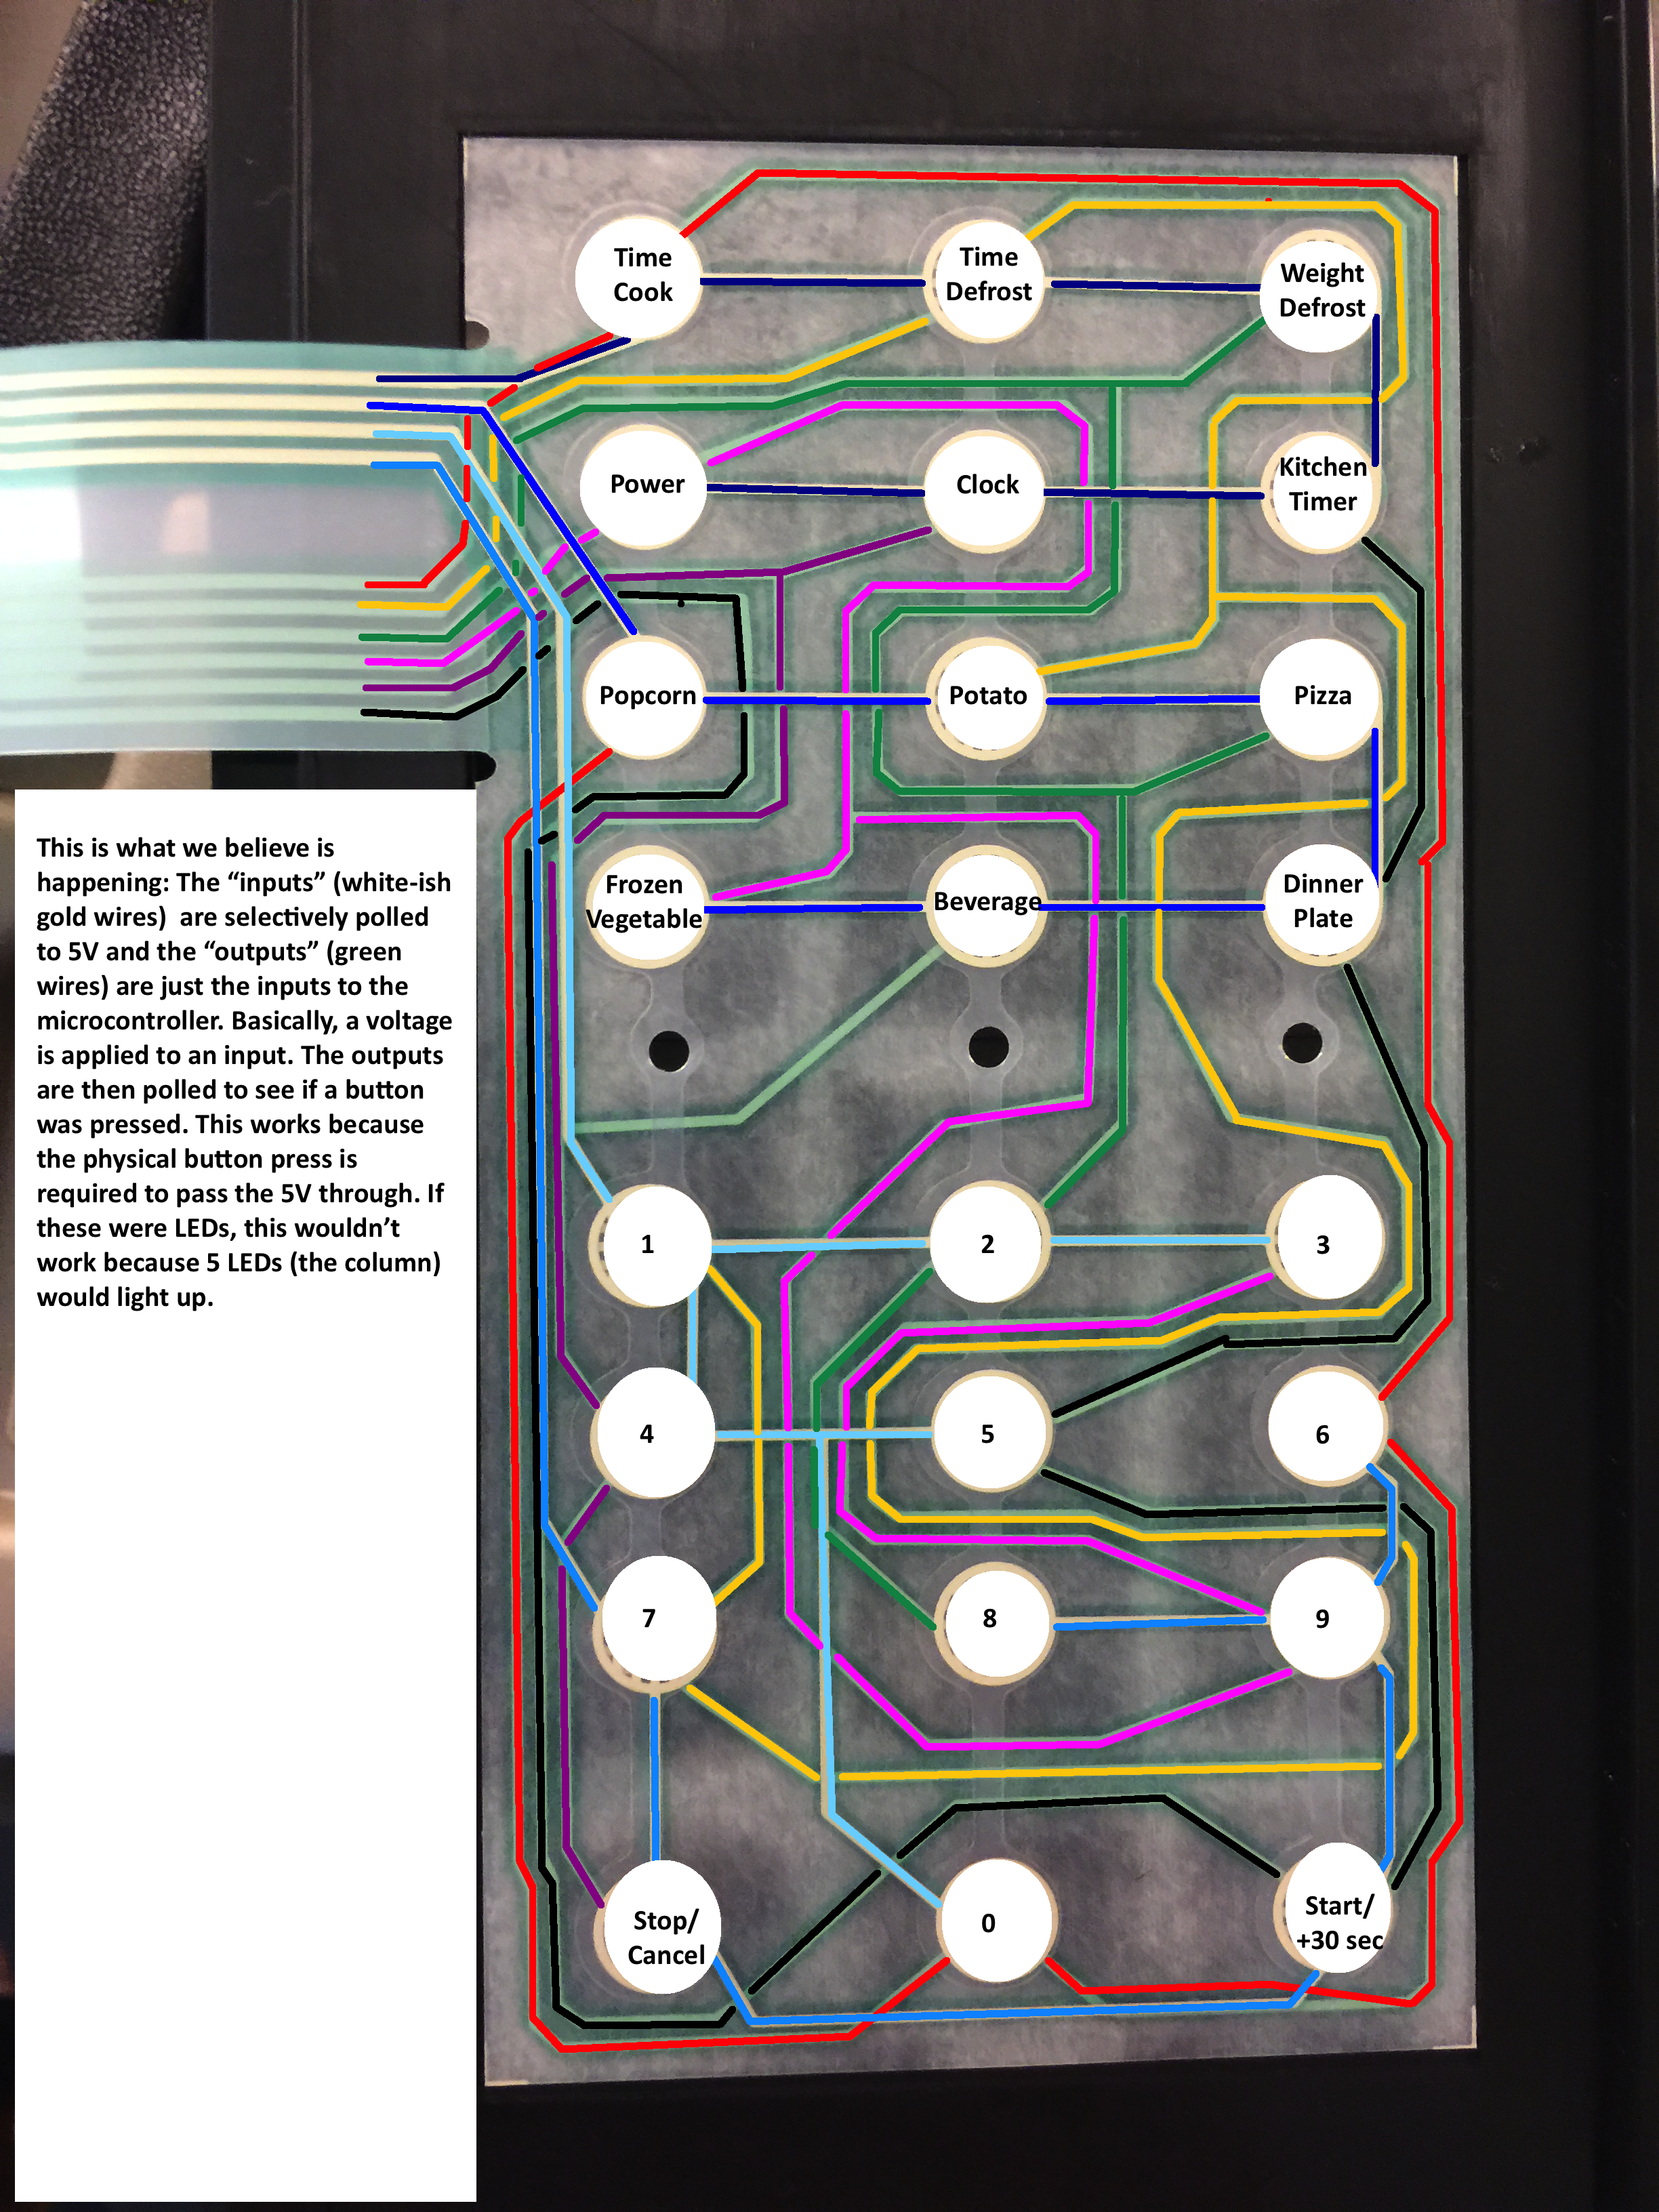
\includegraphics[width=0.5\textwidth]{Button_Matrix_Image.png}
\caption{\label{fig:buttonmatrix}The button matrix map. The top four lines are the output lines, the bottom six are the input lines.  The colors are our own, and show where rows and columns meet to form a single button connection.}
\end{figure}

\subsection*{Arduino}

The heart of our hardware build is an Arduino Uno embedded system platform; it acts as the "brain" of our hardware implementation and decodes instructions from the Android application side of the project \cite{raspberryPicrowaveRepo}.  We chose the Arduino since all of the team members knew it well, and our implementation was well within it's range of capabilities.   The individual pin output mappings from the Arduino, where they go and what they control, are documented in "Button Matrix.txt" \cite{gitHubRepo}.  Wiring the Arduino was one of the simpler aspects of this project.  We also included an RGB LED to indicate communication health, this topic will be covered in more length in the communications section.  The next step was to create a system that the Arduino could control in order to replicate button presses and control the microcontroller.

\begin{figure}[ht]
\centering
\includegraphics[width=.5\textwidth]{Arduino_and_Relay_Board.jpg}
\caption{\label{fig:relay}The Arduino connection to the 16 relay board that we used to control button presses.}
\end{figure}

\subsection*{Relay Board}

In order to imitate button presses, we decided to use a relay board with 16 multipurpose relays built in.  We specifically chose our relay board as it is easily controllable from an embedded system such as an Arduino Uno, which all the team members had substantial experience working with, which made hardware programming and debugging substantially easier.  To map the relays onto the buttons, we arranged them in the same row-column configuration that they are mapped in the matrix.  We did not implement matching relays for all the buttons though, as we deemed some buttons like "popcorn", "potato", "pizza", etc. to be spurious and without project value.  The relay-to-button mappings are also given in the reference file "Button Matrix.txt" \cite{gitHubRepo}.Once the buttons were mapped onto the relay board, we were then able to add two other functional components via the relay board.  First, we changed the motor connection to run through a relay, which gave us the ability to toggle plate rotation as we wished.  Secondly, we added a 12V Xbox fan connected through a relay to the opposite side of the microwave in order to keep our extra componentry cool and to prevent condensation buildup when cooking food.

With the relay board wired up buttons (shown in Figure \ref{fig:arduinorelaywired}), we were able to then create a test system where the Arduino would decode input strings into button presses, and we were able to start controlling the microwave and begin fleshing out the rest of our system.

\begin{figure}[h]
\centering
\includegraphics[width=0.5\textwidth]{ArduinoRelayWired.JPG}
\caption{\label{fig:arduinorelaywired}The Arduino and relay wired into the microwave controller board.}
\end{figure}

\section{Software}

The overall diagram of how the software controls the hardware and microwave is given in Figure \ref{fig:hardwaresoftware}.  With the basic design of how to control the microwave itself done, we were able to design the Android application and the connections between the application and the hardware.  

\subsection*{The Food Information Database}
The first link in our software chain is the remote database that we are using to store information about food to be cooked in the microwave.  In selecting our database type, we recognized that we needed to go with something lightweight and flexible;  our implementation did not require the use of a fully fledged database.  With that, we decided to go with an H2 database engine, which fit all of our requirements.  The database is extremely lightweight, if not incredibly fast, and flexible enough to hold our instruction strings and imaging data.  We installed our database on a team member's personal server.  We then set up the database to be accessible from the web address http://nocomment.sipnswirlutah.com:8082, from which we could access it anywhere. The database followed the structure found in Table \ref{tab:database} in the appendix, with columns to store various instruction information.  The component that slowed our database down the most was the decision to include pictures, which will be explained further in the application section.  We felt that some form of imagery was needed in our application, so we felt that the slowdown was justified.  Some examples of our database entries are found in Figure \ref{fig:databaseentries}

\begin{figure}[h]
\centering
\includegraphics[width=0.5\textwidth]{Database.jpg}
\caption{\label{fig:databaseentries}Example food information rows in our database.}
\end{figure}

\subsection*{Communicating via UART over USB}
Because our system made use of two processing centers, one in the Android device and one in the Arduino, we needed a method of communication between the two.  At the very least, we needed a uni-directional system that would pass data from the Android to the Arduino in order to send instructions strings for controlling the microwave.  This turned out to be a significantly challenging portions of the project.  We attempted various methods of communication, none of which save the final method worked well.  In particular, we felt that we had found a probable solution in transferring data over an audio connection by leveraging our Android device's audio port.  We were able to obtain potential partial audio data transfer files for both Android and Arduino, with a testing application. \cite{audioDataTransfer} This would have had the extra benefit of allowing us to have the USB port on the device left free for device charging or other purposes.  Ultimately though we found that the audio transfer was unusable. For various reasons it had difficulty passing data reliably and was overall a poor implementation method.

Instead, we chose to go with an online library we found by Manuel Di Cerbo from Neuxs-Computing GmbH, Switzerland\cite{uartOverUsbLibrary}. This library gave us the ability to run UART serial communication out over a USB connection directly between the Android device and the Arduino.  Though it meant that we could not use the USB port for other communications while running our application without an extensive rewrite of the data transfer methods, it allowed us to spend time on other crucial parts of the project without having to worry that our communications would drop out or that we would have incorrect data packets being transferred between devices. The library also only provides unidirectional communication from the Android tablet to the Arduino, but this was sufficient for our present needs. 

The library came in two parts.  The first, on the Android side, set up the connection classes necessary for the Android to be able to connect to and use the USB port, as well as giving the necessary data packet functions that we would use to send information.  On the Arduino side, the library gave an example Arduino file with the necessary port information ready.  Another key element of the library was how it helped us use interrupt programming on the Arduino.  The information sent by the Android tablet is stored in memory by the Arduino, and an interrupt is signaled anytime new data is retrieved.  With the interrupt working properly, we were able to retrieve the instruction bytes in the form of strings.

A drawback of the library was that it only allowed for Uni-directional communications.  But otherwise it fulfilled all of our requirements and worked extremely well.

\subsection*{Android Application}

As the overall brains of the project, The general outline of the activity map is given in Figure \ref{fig:activitymap}.

\begin{figure}[ht]
\centering
\includegraphics[width=0.5\textwidth]{MicrowaveActivityMap.png}
\caption{\label{fig:activitymap}Android application state diagram and activity map. The back end classes are utilities referenced in multiple activity states.}
\end{figure}

  A major reason that we decided to go with an Android-based user application was that it allowed our team to program our application in Java for the program itself and XML for our design layout, which was something that several members of our team were proficient in.  It also allowed us to make an app that wasn't platform specific; we were able to get our application to work on several different Android devices with the same results.
  
As an Android based program, our application was built around activities.  The activity map shown in Figure \ref{fig:activitymap} is similar to a state diagram for hardware, each state flows to the next one according to the arrows.  This likewise means that the the map must be traversed in reverse in order to return to the main activity, which is easily doable with the default back-button functionality built into an Android OS.  The activities' functions are as follows:
\begin{itemize}
	\item The \underline{Main Activity} is the starting screen brought up when the application first loads.  It has three selections possible: to search the populated food database list by food name, to search the database by UPC scanning, or to enter a manual control mode. When the application first loads it begins to populate the food data from our remote database in the background.
    \item \underline{Manual Microwave Control} allows the user to control the microwave as if they were pressing the buttons on front of the microwave itself.  In this mode, any instructions sent to the microwave are sent as single instructions, just as a user would press a single button at a time on the microwave in order to program it.  This activity contains a software timer that is closely synced to the microwave in order to show the same cooking time on both displays, and to indicate food is done cooking when the microwave shuts off.
    \item \underline{Search by Name} allows the user to input search parameters in a text field.  The application will then search through its list of populated food items to find potential matches.  For example, a search of "burrito" will return all instances of food names containing the word "burrito", as well as food brands that may include that information as well.  The information returned by this activity then feeds into the Search Results activity.
    \item \underline{Search by UPC} code allows the user to scan a bar code by using the Android device camera, and then searching the populated list for a match.  This functionality was achieved by leveraging a third-party software library called ZXing \cite{upcScanningLibrary}. This library has the ability to scan any of the common UPC codes, as well as QR codes. It does this by image recognition and processing. There is a built-in function that allows an activity to be started for a result, which is the way that we received the data back from the scan. Like Search by Name, this activity sends its result to the Search results activity.  An example of the UPC scanning stage is shown in Figure \ref{fig:upcscan}.

\begin{figure}[ht]
\centering
\includegraphics[width=0.5\textwidth]{UPCScanning.jpg}
\caption{\label{fig:upcscan}The UPC scanning stage of Search by UPC.}
\end{figure}

	\item After finding foods, the application then moves into the \underline{Search Results} activity.  From here, the user may select whichever food they wish to cook from this list, which then invokes the instruction activity.  If no suitable result is found by the user, they may use the Android back button to go back to the prior search stage.
    
    \begin{figure}[ht]
    \centering
    \includegraphics[width=0.5\textwidth]{FoodList.jpg}
    \caption{\label{fig:foodlist}The returned list of food items to select from available on the Search Results activity.}
    \end{figure}

    \item The \underline{Instruction Activity} creates a page display of the food that the user has selected, including a picture (if it exists in the database) and the cooking instructions.
    
    \begin{figure}[ht]
    \centering
    \includegraphics[width=0.5\textwidth]{SelectScreen.jpg}
    \caption{\label{fig:selectscreen}The screen showing the user food information and the automated cooking instructions.}
    \end{figure}
    If the Instruction Activity is entered via the Microwave Running Activity, then it automatically enters the Enjoy Activity.
    
\begin{figure*}[ht]
\centering
\includegraphics[width=1.0\textwidth]{DecodingInstructions.png}
\caption{\label{fig:decodinginstructions}The state diagram of how the Arduino decodes instructions from the application.}
\end{figure*}

	\item Once the user selects "Select" from the Instruction activity, the application will then go into the \underline{Microwave Running Activity}.  On entering this activity, the application automatically sends instructions over the UART connection to the Arduino to program the microwave according to the specifications retrieved from the database.  On selecting "Start", the microwave will then send a signal to the Arduino to start the microwave and a software timer will initiate that matches the timer on the microwave.  Similar to the timer in the Manual Microwave Control activity, the timer is synced to closely match the microwave itself.  On completion of the running activity, control is returned to the parent Instruction Activity.
    \item The \underline{Enjoy Activity} is entered after the microwave running activity completes.  It is simply there to let the user know their food is cooked, or to add an additional 30 seconds if necessary.
\end{itemize}
In addition to the activity states, there are several special classes that our team created that are passed between activities:
\begin{itemize}
  	\item The \underline{Food Item} class contains information pulled from the database and is passed between activities to synchronize what food is being cooked, along with its pertinent information.
  	\item The \underline{Local Database} is the local copy of the database that is referenced when running the application.  All information that is pulled in from the remote database is saved into this local copy, and it is this copy that searching is performed on.
	\item The \underline{USB Singleton} is a very important core class to our entire project. The code (by Manuel Di Cerbo \cite{uartOverUsbLibrary}) that we utilized is viewable on our GitHub repository. It is instantiated only once and referenced by multiple activites, and is the class that passes information from the local database to the Arduino, abstracting away all the otherwise cumbersome USB protocols.  Because this class is so well abstracted, it allowed us to focus more on the implementation of our project and much less on the tedious low-level programming required when dealing with implementing UART-over-USB connections.
\end{itemize}


\subsection*{Instruction Encodings}
As we created our own application of software and hardware in controlling the microwave, it became necessary for us to create our own instruction set for sending instructions to the microwave.  To this purpose, we repurposed and added to a set of encodings that are stored in the database and passed on by the Android application to Arduino in string format.  The Arduino then has the job of interpreting those instructions into button presses via a series of case statements in code \cite{raspberryPicrowaveRepo}.  It was important that our instruction strings and the instruction order match the actual capabilities of the microwave.  Some functions were not available in all modes, such as power modifications at inappropriate times.  Thus we had to make sure that our casing structure was correct in all circumstances.  The encoding interpretations are given below and shown in the Figure  \ref{fig:decodinginstructions} diagram.

\begin{itemize}
	\item 'b' - this character in a string indicates a single button press.  In a string, another single character must immediately follow.
      \begin{itemize}
          \item '0' - '9' - A numeric character indicates that the corresponding number button is to be pressed.
          \item 't' - Press the time cook button.
          \item 'c' - Press the stop/cancel button.
          \item 'p' - press the power button
          \item 's' - press the start button.
      \end{itemize}
    \item 't' - Indicates that the time cook button is to be pressed.  This must be followed by any number of numeric '0'-'9' characters indicating the number of seconds to cook the food.  A non-numeric character acts as the break between the number of seconds to cook and the next instruction.
    \item 'p' - Indicates that the power button is to be pressed, controlling the cooking power of the microwave.  This can be achieved in one of two ways:
    	\begin{itemize}
			\item 'i' - If an 'i' is received, it must then be followed by numeric characters '0' - '1''0', indicating the power level be set between 0 and 10.  This corresponds to the power button being pressed, and then the desired power level being set.
            \item 'l' - The 'l' character indicates that the power level be set to a specific pre-determined value according to the next character received:  
              \begin{itemize}
              		\item 'h' - "High", set to power level 10.
                    \item 'm' - "Medium", set to power level 7.
                    \item 'l' - "Low", set to power level 5.
                    \item 'd' - "Defrost", set to power level 3.
                    \item 'z' - "Zero", set to power level 0.
              \end{itemize}
 		\end{itemize}             
        \item 's' - Indicates that the microwave start button should be pressed and that the cooling fan should be turned on.
        \item 'S' - Indicates that the stop/cancel button should be pressed and the cooling fan should be turned off.
        \item 'm' - Toggles the running of the plate motor.
        \item '\textasciitilde' - This "heartbeat" character is generated and sent once every 1/10th of a second by the Android program to the Arduino.  It indicates that the UART connection between the two devices is still healthy.
        \item 'f' - Indicates the end of an instruction string, and that the Arduino needs to start processing.

\end{itemize}

\subsection*{Arduino Decoding}
The Android sends an instruction string to the Arduino one byte at a time, where it is stored in the UDR0 register.  Whenever that register is changed, the Arduino processor generates an interrupt that indicates that there is new data in that register that needs to be processed immediately.  The byte from that register is then read into a first-in-first-out (FIFO) buffer.  When the Android application is done sending an instruction string, it sends an 'f' character, indicating that the instruction string is complete.  The Arduino then sets a flag in its interrupt method that the main process should start processing the string and translating it into relay switching and button presses.

The Arduino translates the button presses as described above in the encodings section, and in Figure \ref{fig:decodinginstructions}.

Of particular note is the heartbeat character.  It is not ever translated into a message string, and only indicates that the connection between the two devices is still valid.  The Arduino instantiates a timer such that it keeps track of the time received between these pulses.  Whenever this character is received, the Arduino will create a green pulse on the RGB LED to indicate that the connection is working correctly.  It then resets the timer start counting up again.  Should the connection be broken and the heartbeat lost, the timer will continue to count up without being reset.  If a total of five seconds pass without the connection being restored, the Arduino will set the USB to light up red, indicating visually that the connection has been lost.  If a heartbeat is received again, it will begin to flash green again.  This functionality helped us as the designers and testers to keep track of when the connection was active and when it wasn't, and helped us immensely with debugging our communications setup.

\section{Challenges}
As with any major project, it was fraught with plenty of challenges for us to overcome.  

As detailed above, we had to overcome problems in trying to implement a robust communications system.  As we needed to separate the hardware and software to the extent we did, this became an important aspect of our project in making everything in our project cohesive.  As described earlier, we ran into major difficulties in trying to get various forms of communication protocols to work, the most notable being the failed audio transfer \cite{audioDataTransfer}. We also considered wifi and bluetooth as methods of communication, but we found that those protocols were too difficult and time-intensive for our implementation.  In the end, we are grateful for the De Cerbo's UART over USB library that performed exactly the function that we needed.

The application software timers in particular proved to be an persistent problem, as were unable to get decent precision in matching the microwave timers on the application.  We solved this by increasing the precision of our timers to a millisecond scale.  Our timers are still not synced perfectly, as the way that the microwave handles timers is on a hardware level, and is not something that we can replicate with our software timers.  Additionally, consecutive changes to cooking times while the two timers are running cause discrepancies, as the microwave hardware timers both update instantaneously and do a bit-level addition to the timers as they are.  Our software timers require re-instantiations in order to make changes.  While a millisecond timer does much to mitigate our earlier problems, they are not perfect. 

Hardware challenges were thankfully pretty limited, our soldering and wiring worked extremely well.  The problems we did have with hardware stemmed from USB connections being faulty.  Specifically on our demo day, Murphy's law decided to strike by making connecting our application to the hardware flaky due to worn out connectors.  Other than that, our hardware build was remarkably sound.

Finally, we had plans for implementing a thermal camera interface with our application.  One of the stretch goals for the microwave was to include a thermal camera that would improve the functionality of our microwave significantly.

\begin{figure}[h]
\centering
\includegraphics[width=0.5\textwidth]{ThermalCamera.jpeg}
\caption{\label{fig:thermalcam}The Seek Thermal camera mounted on the viewing hole in the microwave.}
\end{figure}

We bought a Seek Thermal camera that was compatible with our Android device, and mounted it on top of a viewing hole in the microwave enclosure.  We made sure that the viewing hole was consistent with the other ventilation holes in the enclosure, ensuring that no microwaves would escape.  We were able to see food heating within the microwave, and it opened up a number of possible features for our application.  Specifically, we were interested in performing analyses on the thermal information pulled from the camera that would have in turn allowed us to cook food in a better way.  These improvements will be described in the Future Improvements section.

What hindered our ability to make the thermal camera useful was that we were not able to get the software development kit from Seek itself.  The kit was supposed to have had a delivery time towards the beginning of our project, and it would have allowed us plenty of time to incorporate information processing on the data.  As of the writing of this paper, that kit is still in development and has not been delivered many months late, and therefore we were not able to incorporate it into our project.  We did attempt to write a USB driver to retrieve information from the camera, but with very limited success.  In the end, we decided to abandon the image processing functionality of the project in favor of making the rest of the application as well polished as we could.

\section{Future Improvements}

We fully acknowledge that our project is in essence only a prototype build.  As we worked on the project, we realized that there were myriad other improvements that could be made to make our project better overall and that would move towards being more of a consumer type product.

\subsection*{Database Extension}
The database needs to be extended so that it can include microwave models, backups of user-specific database alterations, etc. This will allow for product-specific cooking instructions and even allow for small changes like altitude correction, if necessary.
\subsection*{Database Persistence}
Currently, the entire database is dumped onto the device every time that the app is opened. Since the image files are also stored in the database, this download can take quite a long while. We would like to implement a download scheme that allows for an initial dump of data when the app is installed, but then keeps the relevant data on the device until that particular entry is updated on the database.
\subsection*{Database Web Form}
We would like to create a web form that can be accessed by registered companies so that their cooking instructions can be easily entered and updated.
\subsection*{USB Permission Memory Persistence}
We were unable to get the Android tablet to recognize the Arduino bridge as the same USB device each time it was connected, so permission to access the device was requested each time we connected the bridge. We would like to solve this issue so that the permission need only be requested once. 
\subsection*{Bi-directional Communication}
Bi-directional communication would allow data from the Arduino to be sent back to the tablet. This would allow us to know information about the state of the microwave itself, including whether the door was open, if there was a disconnect with the bridge, and data that we can gather through sensors such as temperature, humidity, smoke, etc.
\subsection*{Product-Specific Microcontroller}
Much of the data transfer complexity of the project could be bypassed if a microcontroller were be built into the microwave from the beginning. That way the microwave itself is running code similar to the Arudino code that we have written and wouldn't require USB connections or the like.
\subsection*{Self-Contained System}
We would like to permanently mount the tablet onto the microwave in future editions so that the system is self-contained. This will decrease the change of damage to the system.
\subsection*{Solving the Hot Spot Problem}
The SDK for the Seek Thermal camera was never delivered, so we had no way to extract images or thermal data from the thermal camera. We are interested in integrating this in the future. We will do data analysis on the thermal data or on the image itself in order to more accurately heat food. This will allow for even better food quality because the cold spots in the food could be turned so that they are directly position in the one of the microwave's hot spots, or the opposite for a portion of the food that has gotten too warm.

\subsection*{Integration Into Other Appliances}
This technology could be altered to work in other appliances such as ovens, toaster ovens, crock pots, or even stovetops. With manufacturer-specific cooking instructions for food, the information gathered would allow a change in heat flow in the oven, for example, to heat a colder spot on the Thanksgiving turkey. Additional safety features could also be added such as alerting the cook via alarm or text message if smoke is detected in the oven.

\section{Conclusion and Lessons Learned}
The project came together well and turned out even better than originally planned as the design morphed along the way. The lack of the SDK for the thermal camera didn't allow us to take this as far as we would have liked, but we will continue this work in the future. We think that the product delivered is a very able prototype and that, with the future changes listed above, could become a viable product to take to market. 

In conclusion, our group learned a lot from this project, using the various technologies and methods that we've learned as students to make a prototype consumer product.  We fully believe that the our microwave project showcases all that we've learned as students and that it fulfills the requirements necessary of a good senior project.

\bibliographystyle{IEEEtran}
\bibliography{bibliography}

\section{Appendix}

\subsection*{List of Reference Files}
\begin{itemize}
	\item \underline{Audio Data Transfer}: This method of communication is not used in our project anymore, but was implemented in earlier stages.
    \begin{itemize}
    	\item \underline{Android Code}: Contains Android code for sending data over audio.
    	\item \underline{Arduino Code}: Contains Arduino code for receiving data over audio.
    \end{itemize}
    \item \underline{Construction Images}: Contains images of project construction.
    \item \underline{Microwave Relay}: Contains final Arduino code for our project.
    \item \underline{Seek PC Integration}: Contains Android code for communicating with the Seek Thermal Camera.  We were unable to get this to work, so it is not currently part of our final project.
    \item \underline{Smart Thermal Microwave}: Contains all Android code for our Smart Microwave app.
	\item \underline{Videos}: Contains videos demonstrating our project.
    \item \underline{Other Files}:
    \begin{itemize}
      \item \underline{Button Matrix.txt}: Describes how to interpret the button matrix (found in Construction Images/Button Matrix Image.png).  Also contains information on Arduino pin-outs and relay usage.
      \item \underline{Survey Stats.xlsx}: Shows preliminary survey results in tabular and graphical form.
      \item \underline{Thermal Microwave Presentation.pdf}: Final presentation slides from demo day.
      \item \underline{Weekly\_Log.txt}: Weekly log of the project starting March 29th, 2015.
    \end{itemize}
\end{itemize}

\subsection*{Timeline of Events}
See Weekly\_Log.txt in the resource files for information about project event flow.

\subsection*{Responses to User Survey}
The user survey results can be viewed in their entirety in Survey Stats.xlsx in our resource files, including graphs of results. Some of the changes recommended by the survey were implemented before the final demo day and helped us focus our efforts at the end of the project. The results were all measured on a scale of 1-10, with 1 being the worst and 10 being the best. The condensed results were as follows: 
\begin{itemize}
	\item Functionality of Device: 9.03
	\item Satisfaction with Cooking Results: 8.96
	\item User Interface: 9.23
	\item Overall Satisfaction: 9.08
	\item Would Want for Oneself: 8.08
\end{itemize}
Overall, the response was positive and the participants were excited by the idea of owning one of these devices.

\subsection*{Parts List}
\begin{itemize}
	\item West Bend Microwave
	\item LG GPad 7.0 LTE Tablet running CyanogenMod
	\item Arduino Uno R3
	\item Sainsmart 16-relay Relay Board
	\item Seek Thermal Camera
    \item Acrylic for Display Case
    \item 12v Xbox 360 Fan
    \item Wire, LEDs, cables, etc.
\end{itemize}

\begin{table*}[h]
\centering
{
\rowcolors{2}{gray!10}{gray!30}
\begin{tabular}{| c | c | c | c | c | c | c |}
\hline
\multicolumn{7}{|c|}{DATABASE STRUCTURE}\\
\hline
\ \# & ID\_Number & Food\_Type & Brand\_Name & UPC\_Code & Instructions & Image \\
\hline
\ Info\_Row[0] & & & & & & \\
\hline
\ \dotfill & & & & & & \\
\hline
\ \dotfill & & & & & & \\
\hline
\ \dotfill & & & & & & \\
\hline
\  Info\_Row[x] & & & & & & \\
\hline
\end{tabular}
}
\caption{\label{tab:database}}
\end{table*}

\begin{figure*}[h]
\centering
\includegraphics[width=1.0\textwidth]{TeamPhoto.jpeg}
\caption{\label{fig:teamphoto}The members of Team Smart Microwave are, from left to right, James Watts, Darin Stoker, and Stuart Johnsen.}
\end{figure*}

\end{document}